% This is auto-generated file: do not edit!
% Exported from microMathematics Plus, version 2.20.0


Este app é um poderoso programa
calculador em formato de folha de
cálculos. A folha de cálculos pode ser
editada livremente, armazenada no
cartão SD, aberta de um cartão SD e
exportada para uma imagem ou formato
LaTeX.

A folha de cálculos é um documento
matemático que contém texto, fórmulas
e gráficos. Ela suporta edição em
tempo real de notações matemáticas e
seu cálculo automático.

Os objetos a seguir podem ser
inseridos na folha de cálculos:
equações, janelas de resultado,
gráficos, fragmentos de textos e
imagens. Este documento fornece uma
visão geral de como editar estes
objetos.

\subsection{Edição}

Quase todos os objetos disponíveis
possuem vários campos editáveis. Para
editar o campo use os símbolos e
funções na barra de ferramentas.

Todos os símbolos podem ser entrados
pelo teclado. Para encontrar qual
símbolo do teclado corresponde ao
símbolo matemático que você deseja,
leia a dica segurando o botão de
interesse.

Ao segurar em um termo você pode
selecionar este termo. O termo
selecionado pode ser excluído, copiado
para a área de transferência, colado
da área de transferência ou outra
operação ou função pode ser inserida
depois do termo usando os botões da
barra de ferramentas ou teclado.

O comando ''Desfazer'' está disponível
na barra de ações. Ele apaga a última
mudança feita ao documento e reverte-a
para um estado anterior:
\begin{center}\begin{tabular}{c} 
\includegraphics[width=0.45\textwidth]{graphics/how_to_use_fig1.png} \end{tabular}\end{center}

\subsection{Equação}

Uma equação define uma constante
numérica, um intervalo ou uma função.
Para criar uma equação, use o botão
''Novo elemento'' na barra de ações
\begin{center}\begin{tabular}{c} 
\includegraphics[width=0.45\textwidth]{graphics/how_to_use_fig2.png} \end{tabular}\end{center}

ou o botão ''Adicionar equação'' da barra
de ferramentas:
\begin{center}\begin{tabular}{c} 
\includegraphics[width=0.45\textwidth]{graphics/how_to_use_fig3.png} \end{tabular}\end{center}

Uma equação com dois campos vazios
aparece. Estes campos devem ser
preenchidos:
\begin{center}\begin{tabular}{c}
  ${\Box} := {\Box}$
\end{tabular}\end{center}

O nome da equação é dado no campo
esquerdo. O nome deve conter letras ou
dígiros apenas e srá usado em outros
objetos para referenciar esta equação.

A partir da barra de ações, você pode
abrir a janela de ''Configurações do
documento'': 
\begin{center}\begin{tabular}{c} 
\includegraphics[width=0.45\textwidth]{graphics/how_to_use_fig4.png} \end{tabular}\end{center}

Dependendo do parâmetro ''Permitir
re-definir equações'' nesta janela, há
dois modos de uso:

a) se a redefinição não for permitida,
o nome da equação deve ser único
dentro de todo o espaço de trabalho e
a equação pode ser usada antes e
depois de ser definida,

b) se a redefinição for permitida,
você pode redefinir mais de uma
equação com o mesmo nome. Se esta
equação está referenciada, a última
versão definida antes de chamar a
função será usada.

\subsubsection{Constante}

Se o nome da equação não contém nenhum
argumento entre parênteses, isso
define uma constante ou um intervalo:
\begin{center}\begin{tabular}{ccc}
  $N := 200$ &
  $Sq2 := \sqrt{100} $ &
  $Pi2 := \frac{{\pi}}{2}$ \cr
\end{tabular}\end{center}

Neste último exemplo, uma constante
embutida pi foi usada. Atualmente, as
seguintes constantes embutidas estão
disponíveis:
\begin{center}\begin{tabular}{ccc}
  ${\pi} = 3.14159$ &
  $pi = 3.14159$ &
  $e = 2.71828$ \cr
\end{tabular}\end{center}

Uma constante definida anteriormente
também pode ser usada:
\begin{center}\begin{tabular}{c}
  $NPi2 := N \cdot Pi2$
\end{tabular}\end{center}

Você também pode usar o símbolo ''i''
como unidade imaginária para poder
definir um número complexo:
\begin{center}\begin{tabular}{c}
  $z := 5 + 3i$
\end{tabular}\end{center}

\subsubsection{Intervalo}

Uma equação do tipo intevalo define uma
variável qur foi alterada de um valor
minímo dado até um valor máximo dado
com incremento definido. Esta variável
pode ser usada como o argumento do
gráfico de uma função ou como um
parâmetro para construir uma tabela de
valores da função.

Para definir um intervalo, insira um
nome válido no lado esquerdo de uma
equação vazia. No lado direito desta
equação, coloque um símbolo '':'', ou
toque no botão ''Intervalo
equidistante'' da barra de ferramentas:
\begin{center}\begin{tabular}{c} 
\includegraphics[width=0.45\textwidth]{graphics/how_to_use_fig5.png} \end{tabular}\end{center}

Aqui, o primeiro elemento é o ponto
inicial do intervalo, o próximo
elemento é o segundo ponto, e o último
elemento é o ponto final do intervalo:
\begin{center}\begin{tabular}{c}
  $x := \left[ 0,\, 0.1 \,..\, 10 \right]$
\end{tabular}\end{center}

Os elementos do intervalo podem ser
acessados como segue:
\begin{center}\begin{tabular}{ccc}
  $x_{0}  = 0.0$ &
  $x_{1}  = 0.1$ &
  $x_{100}  = 10.0$ \cr
\end{tabular}\end{center}

O incremento é a diferença entre o
segundo e o primeiro valores:
\begin{center}\begin{tabular}{c}
  $x_{2}  - x_{1}  = 0.1$
\end{tabular}\end{center}

Por exemplo, podemos definir um
intervalo equidistante que contém N
pontos distribuídos com incremento
''dy'' onde o início do intervalo é zero
como segue:
\begin{center}\begin{tabular}{cc}
  $dy := 0.05$ &
  $y := \left[ 0,\, dy \,..\, dy \cdot N \right]$ \cr
\end{tabular}\end{center}

\subsubsection{Function}

Uma função é uma relação entre um ou
mais argumentos e um conjunto de
saídas permissivas com a propriedade,
que cada valor do argumento (real ou
complexo) ou a combinação de
argumentos está relacionada à
exatamente uma saída.

O nome da função e o argumento entre
parênteses são dados no lado esquerdo
da equação. Não é necessário definir o
argumento na folha de trabalho
anteriormente, você pode definí-lo
como quiser, mas usando apenas letras
ou dígitos:
\begin{center}\begin{tabular}{c}
  $f(t) := sin \left( t\right)  \cdot cos \left( t\right)  / 2$
\end{tabular}\end{center}
\begin{center}\begin{tabular}{c}
  $w(z) := {e}^{2i \cdot {\pi} \cdot z}$
\end{tabular}\end{center}
\begin{center}\begin{tabular}{c}
  $H(x,y) := \sqrt{{x}^{2} + {y}^{2}} $
\end{tabular}\end{center}
\begin{center}\begin{tabular}{c}
  $g(x,y) := \frac{sin \left( H \left( x,\, y\right) \right) }{H \left( x,\, y / 2\right)  + 1}$
\end{tabular}\end{center}

O lado direito da função contém uma
fórmula matemática de como calcular a
função. Se esta fórmula não contém o
argumento da função declarado, tal
função será interpretada como uma
constante.

Você também pode usar o lado direito
ou outras funções embutidas ou
previamente definidas. Para inserir um
função entre o nome dela, toque no
abre parênteses
 ''('' e então entre o argumento. Este
argumento também pode ser uma fórmula,
que contém quaisquer outras operações
e funções.

\subsubsection{Array}

Arranjos são funções especiais com as
seguintes propriedades:

a) apenas um intervalo previamente
definido pode ser usado como um
argumento de arranjo:
\begin{center}\begin{tabular}{cc}
  $k := \left[ 0,\, 1 \,..\, 100 \right]$ &
  $m := \left[ 0,\, 1 \,..\, 200 \right]$ \cr
\end{tabular}\end{center}

a) argumentos de arranjos são dados
entre [ ] ao invés de ( ):
\begin{center}\begin{tabular}{c}
  $M[k,m] := {sin \left( k / 10\right) }^{2} - 3 \cdot  \left| cos \left( m / 10\right)  \right| $
\end{tabular}\end{center}

c) elementos de arranjos são calculados
e armazenados na memória que reduz o
tempo de acesso à esses valores

d) elementos de arranjos podem ser
acessados apenas usando um índice
menor. Para criar um índice menor,
coloque ''['' após o nome do arranjo:
\begin{center}\begin{tabular}{cc}
  $M_{5,\, 10}  = -1.39106$ &
  $M_{10,\, 5}  = -1.92467$ \cr
\end{tabular}\end{center}
\begin{center}\begin{tabular}{c}
  $P[k,m] := floor \left( -10 \cdot M_{k,\, m} \right) $
\end{tabular}\end{center}

e) se qualquer índice do arranjo for
complexo ou negativo ou maior que o
limite superior do intervalo
correspondente, o número inválido será
retornado:
\begin{center}\begin{tabular}{cc}
  $M_{10i,\, 100}  = NaN$ &
  $M_{90,\, 210}  = NaN$ \cr
\end{tabular}\end{center}

\subsection{Result View}

Este elemento é usado para representar
um resultado de cálculo como um número
ou uma tabela. Para adicionar este
elemento, use o botão ''Novo elemento''
na barra de ações ou o botão
''Adicionar janela de resultado'' da
barra de ferramentas:
\begin{center}\begin{tabular}{c} 
\includegraphics[width=0.45\textwidth]{graphics/how_to_use_fig6.png} \end{tabular}\end{center}

Uma equação com dois campos aparece,
onde o campo esquerdo deve ser
preenchido:
\begin{center}\begin{tabular}{c}
  ${\Box} = {\Box}$
\end{tabular}\end{center}

O termo da esquerda contém uma fórmula
para ser calculada e o termo da
direita é o resultado do cálculo. O
resultado será mostrado quando você
pressionar o botão flutuante
''Calcular''.

No termo da esquerda você pode usar
quaisquer constantes e funções
definidas previamente assim como
quaisquer funções embutidas:
\begin{center}\begin{tabular}{c}
  ${e}^{{\pi}} \cdot f \left( NPi2\right)  = 2.27286E-14$
\end{tabular}\end{center}

Se a parte da esquerda não contém
nenhuma variável ''parecida com
intervalo'', o resultado do cálculo é
apenas um número real ou complexo:
\begin{center}\begin{tabular}{c}
  $y_{N - 1}  - y_{0}  = 9.95$
\end{tabular}\end{center}
\begin{center}\begin{tabular}{ccc}
  $\Re\left( z \right)  = 5.0$ &
  $\Im\left( z \right)  = 3.0$ &
  $ \left| z \right|  = 5.83095$ \cr
\end{tabular}\end{center}
\begin{center}\begin{tabular}{c}
  $\sqrt{sin \left( \frac{3}{2} \cdot {\pi}\right) }  = 0.0+1.0i$
\end{tabular}\end{center}

Se a parte da esquerda contém uma
variável de intervalo, o resultado do
cálculo será um vetor de valores
correspondentes à este intervalo.
Devido ao limite de espaço livre na
tela, apenas os primeiros e últimos
elementos do vetor serão exibidos:
\begin{center}\begin{tabular}{ccc}
  $x = \begin{bmatrix}0.0\\0.1\\0.2\\0.3\\0.4\\0.5\\\dots\\10.0\\\end{bmatrix}$ &
  $y = \begin{bmatrix}0.0\\0.05\\0.1\\0.15\\0.2\\0.25\\\dots\\10.0\\\end{bmatrix}$ &
  $2 \cdot y = \begin{bmatrix}0.0\\0.1\\0.2\\0.3\\0.4\\0.5\\\dots\\20.0\\\end{bmatrix}$ \cr
\end{tabular}\end{center}
\begin{center}\begin{tabular}{c}
  $P_{k,\, m}  = \begin{bmatrix}30.0&29.0&29.0&28.0&\dots&12.0\\29.0&29.0&29.0&28.0&\dots&12.0\\29.0&29.0&29.0&28.0&\dots&11.0\\29.0&28.0&28.0&27.0&\dots&11.0\\\dots&\dots&\dots&\dots&\dots&\dots\\27.0&26.0&26.0&25.0&\dots&9.0\\\end{bmatrix}$
\end{tabular}\end{center}

Número de elementos exibidos e o modo
no qual o resultado é exibido podem
ser alterados. Segurando na área da
fórmula e o menu de contexto,
selecione a fórmula toda. Se a fórmula
está selecionada, o botão flutuante
''Propriedades do objeto'' aparece. Se
você tocar neste botão, o a janela de
propridades do resultado será exibida:
\begin{center}\begin{tabular}{c} 
\includegraphics[width=0.45\textwidth]{graphics/how_to_use_fig7.png} \end{tabular}\end{center}

O segundo botão flutuante, ''Detalhes'',
também aparecerá. Se você tocar neste
botão, a janela de ''Detalhes'' será
exibida, onde você pode observar todos
elementos do arranjo.

Note que o uso de três ou mais
variáveis-intervalo no lado esquerdo
da visualização não é permitido nesta
versão do app.

\subsection{Desenho de Função}

O elemento de desenho de função exibe
um gráfico de uma função, que depende
de um único argumento. Para criar um
desenho, use o botão ''Novo elemento''
na barra de ações ou o botão
''Adicionar desenho de função'' na barra
de ferramentas:
\begin{center}\begin{tabular}{c} 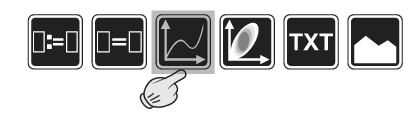
\includegraphics[width=0.45\textwidth]{graphics/how_to_use_fig8.png} \end{tabular}\end{center}

O painel de desenho com seis campos
vazios aparece. A função a ser
desenhada deve ser colocada no campo
central-esquerdo e o argumento da
função no campo central-inferior:
\begin{center}\begin{tabular}{c} 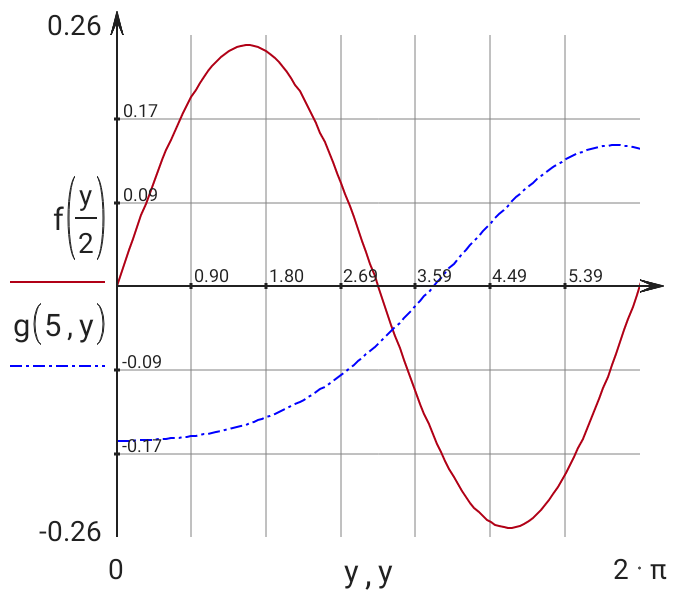
\includegraphics[width=0.45\textwidth]{graphics/how_to_use_fig9.png} \end{tabular}\end{center}

Para mais detalhes veja exemplos de
''Desenho de função'' e ''Desenho de
Função Polar'' da gaveta de navegação
do app.

\subsection{Desenho Tridimensional}

O desenho 3D exibe um gráfico de uma
função única que depende de dois
argumentos. Para criar tal desenho,
use o botão ''Novo elemento'' na barra
de açõesou o botão ''Adicionar desenho
3D'' da barra de ferramentas:
\begin{center}\begin{tabular}{c} 
\includegraphics[width=0.45\textwidth]{graphics/how_to_use_fig10.png} \end{tabular}\end{center}
\begin{center}\begin{tabular}{cc}
  $x := \left[ -10,\, -9.5 \,..\, 10 \right]$ &
  $y := \left[ -10,\, -9.5 \,..\, 10 \right]$ \cr
\end{tabular}\end{center}
\begin{center}\begin{tabular}{c} 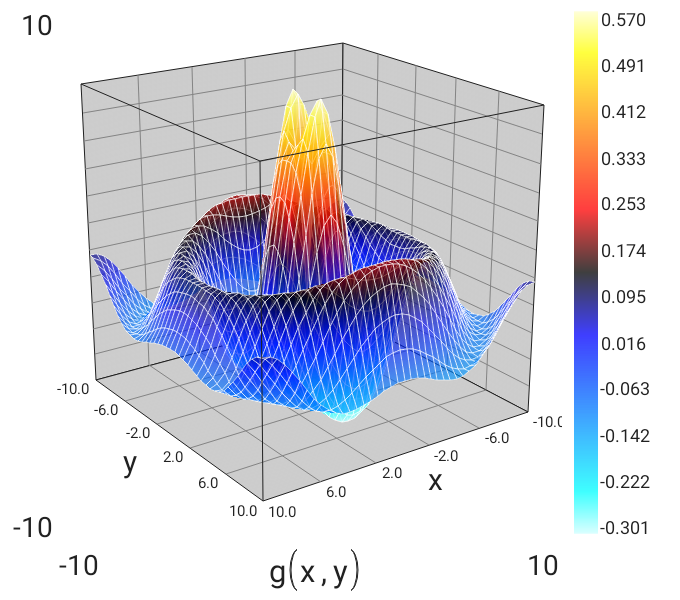
\includegraphics[width=0.45\textwidth]{graphics/how_to_use_fig11.png} \end{tabular}\end{center}

In the center-bottom field, put the
function name or an equation that
contains exactly two previously
defined intervals. The use of an array
is also possible:
\begin{center}\begin{tabular}{c} 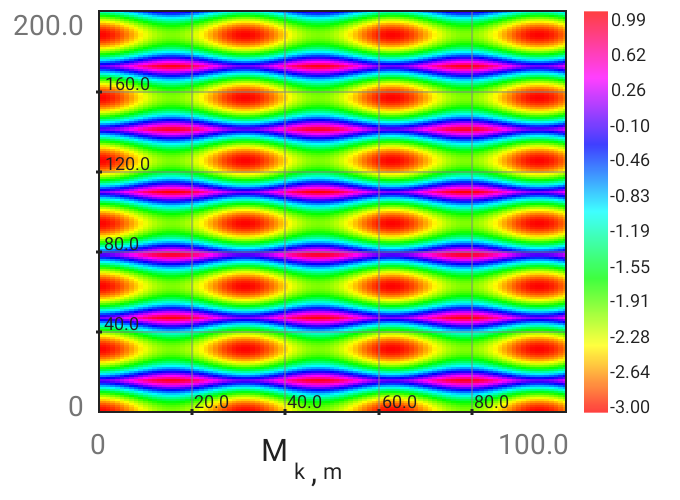
\includegraphics[width=0.45\textwidth]{graphics/how_to_use_fig12.png} \end{tabular}\end{center}

Para mais detalhes veja o exemplo
''Desenho 3D'' da gaveta de navegação do
app.

\subsection{Text Fragment}

O fragmento de texto exibe texto
simples como este. Para adicionar um
fragmento de texto, use o botão ''Novo
elemento'' na barra de ações ou o botão
''Adicionar fragmento de texto'' da
barra de ferramentas:
\begin{center}\begin{tabular}{c} 
\includegraphics[width=0.45\textwidth]{graphics/how_to_use_fig13.png} \end{tabular}\end{center}

Se todo o texto dentro de um fragmento
está selecionado usando o menu de
contexto ''Selecionar tudp'', um botão
flutuante ''Propriedades do objeto''
aparece na parte inferior-esquerda da
tela.

Se você tocar neste botão. a janela
''Propriedades do Texto'' será exibida,
onde você pode selecionar a aparência
do texto e ativar a numeração. Por
exemplo, os títulos neste documento
tem a aparência ''Subsection'' com a
numeração ativada.

\subsection{Image}

Você também pode inserir uma imagem de
um arquivo de imagem. Para fazer isso,
use o botão ''Novo elemento'' da barra
de ações ou o botão ''Adicionar arquivo
de imagem'' da barra de ferramentas:
\begin{center}\begin{tabular}{c} 
\includegraphics[width=0.45\textwidth]{graphics/how_to_use_fig14.png} \end{tabular}\end{center}

A janela de ''Configurações da imagem''
irá aparecer. Nela você pode
selecionar um arquivo com a imagem a
ser inserida e definir o tamanho
necessário da imagem.

Os formatos de imagem a seguir são
suportados: png, bmp, gif, jpeg, svg.

Se você ativar a ''Imagem embutida'' na
janela de ''Configurações de imagem'',
então a imagem será anexada
diretamente no seu documento. Imagem
anexada resulta em um documento único,
mas maior.

Se a ''Imagem embutida'' não estiver
marcada, o arquivo de imagem será
apenas referenciado do que anexado,
i.é. seu documento referencia o
arquivo de imagem fora do documento.
Se você quiser mover seu documento por
favor não esqueça de mover o arquivo
de imagem também.

Você pode alterar as propriedades de
uma imagem já existente. Segure na
área da imagem até que apareça o botão
flutuante ''Propriedades do objeto''. Se
você pressionar este botão, uma janela
com as propriedades da imagem será
exibida.